% Willingness-to-pay step curve, reservation prices and market price
\documentclass[tikz,border=4pt]{standalone}
\renewcommand\familydefault{\sfdefault}
\usetikzlibrary{arrows.meta}
\definecolor{surplus}{RGB}{0,0,230}
\definecolor{cost}{RGB}{255,255,0}
\definecolor{price}{RGB}{60,190,60}
\definecolor{callout}{RGB}{204,204,255}
\begin{document}
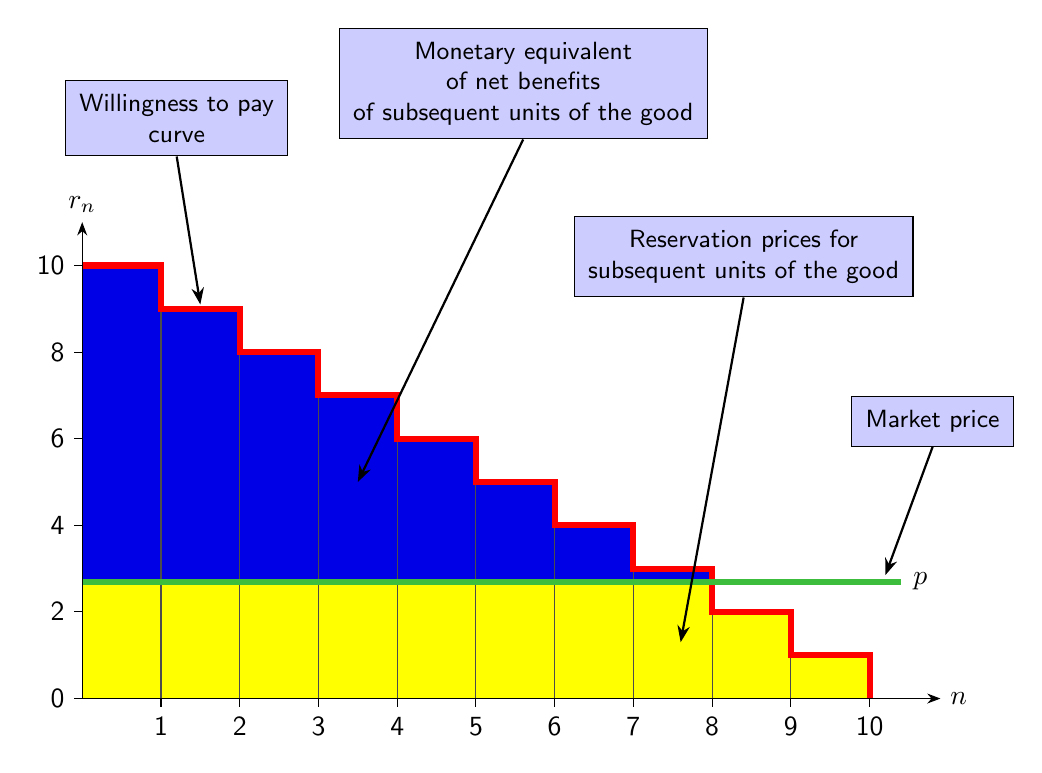
\begin{tikzpicture}[x=1cm, y=0.55cm,
    note/.style={draw, fill=callout, align=center, inner sep=5pt, font=\small},
    pt/.style={-{Stealth[length=6pt]}, thick}]
  \def\p{2.7}
  % bars: unit n has reservation price 11-n
  \foreach \n in {1,...,10}{
    \pgfmathsetmacro\r{11-\n}
    \pgfmathsetmacro\top{min(\r,\p)}
    \fill[cost] (\n-1,0) rectangle (\n,\top);
    \ifdim \r pt > \p pt
      \fill[surplus] (\n-1,\p) rectangle (\n,\r);
    \fi
  }
  \foreach \n in {1,...,9} \draw[black!70] (\n,0) -- (\n,11-\n-1);
  % WTP step curve
  \draw[red, line width=2.2pt]
    (0,10) -- (1,10) -- (1,9) -- (2,9) -- (2,8) -- (3,8) -- (3,7) -- (4,7) -- (4,6)
    -- (5,6) -- (5,5) -- (6,5) -- (6,4) -- (7,4) -- (7,3) -- (8,3) -- (8,2) -- (9,2)
    -- (9,1) -- (10,1) -- (10,0);
  % market price
  \draw[price, line width=2.2pt] (0,\p) -- (10.4,\p) node[right, black] {$p$};
  % axes
  \draw[-{Stealth}] (0,0) -- (10.9,0) node[right] {$n$};
  \draw[-{Stealth}] (0,0) -- (0,11)   node[above] {$r_n$};
  \foreach \n in {1,...,10} \draw (\n,0) -- (\n,-0.2) node[below] {\n};
  \foreach \y in {0,2,...,10} \draw (0,\y) -- (-0.1,\y) node[left] {\y};
  % callouts
  \node[note] (wtp) at (1.2,13.4) {Willingness to pay\\curve};
  \draw[pt] (wtp.south) -- (1.5,9.1);
  \node[note] (cs)  at (5.6,14.2) {Monetary equivalent\\of net benefits\\of subsequent units of the good};
  \draw[pt] (cs.south) -- (3.5,5);
  \node[note] (res) at (8.4,10.2) {Reservation prices for\\subsequent units of the good};
  \draw[pt] (res.south) -- (7.6,1.3);
  \node[note] (mp)  at (10.8,6.4) {Market price};
  \draw[pt] (mp.south) -- (10.2,\p+0.15);
\end{tikzpicture}
\end{document}
